\subsection{Idea general del problema}
Se ha decidido conectar telegráficamente todas las estaciones de un sistema férreo que recorre el país en abanico con origen en la capital (el kilómetro 0). Se nos ofrece cierta cantidad de kilometros de cable para conectar la ciudades de cada ramal. Al ser escaso el presupuesto, se busca lograr conectar la mayor cantidad de ciudades con los metros asignados, sin hacer cortes en el cable. \\
$~~~~~$Se nos propone resolver cuántas ciudades se pueden conectar para cada ramal, con una complejidad de O(n), siendo n la cantidad de estaciones en cada ramal.\\
$~~~~~$Para ello se nos brinda un archivo de entrada, el cual tiene para cada ramal dos líneas: la primera contiene un entero con los kilómetros de cable dedicados al ramal y la segunda los kilometrajes de las estaciones en el ramal sin considerar el 0. Luego de ejecutar nuestro algoritmo, la salida del mismo debe contener, para cada ramal de la entrada, una línea con la cantidad de ciudades conectables encontradas.\\

Un ejemplo de archivo de entrada puede ser, (extracto del archivo Tp1Ej1.in):\\
6 \\
6 8 12 15 \\
35 \\
8 14 20 40 45 54 60 67 74 89 99 \\
100 \\
35 87 141 163 183 252 288 314 356 387 \\
90 \\
6 8 16 19 28 32 37 45 52 60 69 78 82 \\

El mismo indica, en su primer línea que para el ramal 1 tenemos 6km de cable, y en su segunda línea que dicho ramal contiene (además de la capital, implícita, en el kilómetro 0) una estación en el kilómetro 6, otra en el 8, otra en el 12 y la última en el kilómetro 15. Luego para el ramal 2, tenemos 35 kilómetros de cable, y estaciones en los kilómetros: 8 14 20 40 45 54 60 67 74 89 y 99. Así sucesivamente para el resto de los ramales.\\
$~~~~~$El archivo de salida luego de ejecutarse nuestro algoritmo deberá ser de la siguiente pinta, (extracto del archivo Tp1Ej1.out):\\
3 \\
6 \\
4 \\
14 \\

Este último archivo indica la cantidad de ciudades que se pueden conectar para cada ramal. En el caso del ramal 1, para el cual se tienen 6km de cable disponibles, y contiene ciudades en los kilómetros: 0 6 8 12 15 vemos que la solución debería ser que se pueden conectar como máximo 3 ciudades, a continuación explicaremos cómo se deduce esto.\\

Si conectamos la capital con la ciudad del kilómetro 6, al tener sólo 6km de cable, nuestra solución sería que pudimos conectar sólo 2 ciudades. Pero como debemos maximizar esta cantidad, podemos ver que si en vez de conectar a la capital con la primer estación del ramal, conectamos la ciudad del kilómetro 6, con su siguiente y con la del kilómetro 12, entonces como entre el kilómetro 6 y el 8 hay una diferencia de 2kms y entre el 8 y el 12 una diferencia de 4kms, vemos que la máxima cantidad de estaciones conectadas con 6km de cable para el ramal 1, es 3. La misma lógica se la aplica para los ramales restantes.\\

\subsection{Explicación y pseudocódigo}

El algoritmo empieza ubicando dos índices en la primera ciudad, ``start" $ $y ``actual" $ $. Luego, si alcanza el cable, avanza ``actual"$ $ hasta la segunda ciudad, y le resta al cable esa distancia (entre la primer ciudad y la segunda), asi continúa (restando la distancia entre la tercera y la segunda, luego entre la cuarta y la tercera, etc.) hasta que ya no se puedan conectar mas ciudades, esto ocurre cuando el cable pasa a ser negativo. Cada vez que una nueva ciudad es conectada, la variable ``conectadas" $ $ aumenta en uno y se aumenta en uno el indice ``actual"$ $, en caso de llegar a la última ciudad (cuando ``actual"$ $ apunta a la ultima ciudad) termina y retorna la variable ``restemp" $ $ que es igual a ``$ $conectadas" $ $ . Si no, calcula la distancia entre la ciudad apuntada por ``start" $ $ y su siguiente, esa distancia se le suma al resto del cable que quedo disponible y avanza el indices ``start" $ $, ademas le resta uno a la variable ``$ $conectadas" $ $ (siempre que esta sea mayor a 0) pues este proceso simboliza que una ciudad fue desconetada. Con esta nueva cantidad de cable se fija ahora si se puede avanzar más el puntero ``actual"$ $ , repitiendo el proceso de restarle al cable la distancia entre la última ciudad conectada (apuntada por ``actual"$ $) y su siguiente. Este proceso se repite hasta que se termine el cable otra vez (repitiendo el proceso anterior) o se llegue a la última ciudad. Si cuando se termina el cable o se llega al final, el valor de ``conectadas" $ $ es mayor que ``restemp" $ $, se actualiza ``restemp" $ $.

A continuación mostramos un pseudocódigo de la implementación explicada anteriormente. \\

int conectar(vector$<$int$>$ v , int cable) \{ \\
$~~~~~~~~~~~~$int resTemp $\leftarrow$ 0 \Ode{1}\\
$~~~~~~~~~~~~$int start $\leftarrow$ 0 \Ode{1}\\
$~~~~~~~~~~~~$int actual $\leftarrow$ 0 \Ode{1}\\
$~~~~~~~~~~~~$int aux $\leftarrow$ 0 \Ode{1}\\
$~~~~~~~~~~~~$\textbf{mientras} (actual no apunte al último elemento del vector) \{   \Ode{n} \\
$~~~~~~~~~~~~~~~$\textbf{mientras}(cable $\geq$ 0 y actual no apunte al ultimo elemento del vector) \{  \Ode{cable} \\
$~~~~~~~~~~~~~~~~~~~~$Guardamos en aux el cable, por si este pasa a ser negativo \Ode{1}\\
$~~~~~~~~~~~~~~~~~~~~$Le restamos al cable la distancia entre lo apuntado por actual y su siguiente; \Ode{1}\\
$~~~~~~~~~~~~~~~~~~~~$\textbf{si} (longitud del cable $\geq$ 0) \{  \Ode{1}\\
$~~~~~~~~~~~~~~~~~~~~~~~~~~$Incrementamos conectadas en 1 y avanzamos el puntero actual \Ode{1}
$~~~~~~~~~~~~~~~~~~~~$\} \\
$~~~~~~~~~~~~~~~~~~~~$Si conectadas es igual a uno se lo cambia por dos;  \Ode{1}\\
$~~~~~~~~~~~~~~~~$\}\\
$~~~~~~~~~~~~~~~$Si el cable en negativo, se actualiza su valor por el de aux\\
$~~~~~~~~~~~~~~~~~~$Si conectadas es mayor que restemp se actuliza el valor de restemp por el de conectadas\\
$~~~~~~~~~~~~~~~$\textbf{si}(resTemp == 0) \{  \Ode{1} \\
$~~~~~~~~~~~~~~~~~~~~$Conectadas  $\leftarrow$ 0; \Ode{1}\\
$~~~~~~~~~~~~~~~~~~~~$Avanzamos los dos indices, start y acutal;  \Ode{1}\\
$~~~~~~~~~~~~~~~$\} \textbf{si no} \{ \\
$~~~~~~~~~~~~~~~~~~~~$Decrementamos conectadas en 1, ya que desconectamos la primer ciudad \\
$~~~~~~~~~~~~~~~~~~~~$Sumamos al cable la distancia entre lo apuntado por start y su siguiente;\de{1}\\
$~~~~~~~~~~~~~~~~~~~~$Incrementamos start en 1;  \Ode{1}\\
$~~~~~~~~~~~~~~~$\} \\
$~~~~~~~~~~~~$\} \\
$~~~~~~~~~~~~$Devolvemos restemp, en caso de que sea uno, se cambia su valor por dos; \Ode{1} \\
\}\\

\subsection{Deducción de la cota de complejidad temporal y correctitud}

Dedujimos que el algoritmo indica cuantas ciudades se pueden conectar para cada ramal en O(n), siendo n la cantidad de estaciones en cada ramal. El algoritmo termina cuando el segundo puntero, ``actual"$ $, llega al final. Para esto cuenta con dos ciclos (explicados anteriormente), el primero se ejecuta como mucho n veces, ese  caso ocurre cuando se da un cable muy corto y en cada iteración se avanzan los dos índices solo en uno, pasando asi por todos los elementos, en este caso el segundo while solo iteraria una vez pues el cable pasaria a ser negativo instantaneamente, por otro lado el primer while podria llegar a ejecutarse solo una vez si se da un cable muy largo, en este caso el segundo while es el que iteraria n veces, llevando el puntero ``actual"$ $ hasta el final, pero sin mover ``start"$ $ por lo que seria considerado como el mejor caso, aunque este tambien tiene una complejidad O(n).\\
En otro caso, el segundo while del algoritmo se ejecuta mientras que la longitud del cable sea positiva y el indice ``actual"$ $ no apunte a la ultima ciudad, este es el ciclo que va sumando ciudades al ramal y guarda cuantas ciudades se conectaron. Mientras que va conectando ciudades, el algoritmo avanza el segundo puntero, cuando el cable pasa a ser negativo recien ahi se avanza el primer puntero  ,``start"$ $,  suma esa diferencia al cable, se fija si hay que actualizar el resultado, y vuelve a comenzar el segundo ciclo. Este procezo continua hasta que ``actual"$ $ apunte a la ultima ciudad. Notar que en cada iteracion, ``actual"$ $ no siempre avanza, pero cuando no avanza, ``start"$ $ si lo hace y si ``start"$ $ llega a alcanzaz a ``actual"$ $ , en la proxima iteracion ,si ``start"$ $ vuelve a avanzar, lo empuja. Aca se puede obervar el peor caso, que ocurre cuando ``actual"$ $ llega hasta cierto punto arbitrario, y luego ``start"$ $ lo alcanza, si esto pasa todo el tiempo, se recorreria linealmente el vector dos veces, y aunque sigue siendo O(n), es el caso que mas iteraciones produce y por eso es considerado el peor caso.

El algoritmo termina cuando el segundo puntero llega al final, en cada iteración el segundo puntero, ``actual"$ $ avanza en uno, y cuando no avanza, avanza ``start"$ $  tambien en uno. Notar que si ``start"$ $ alcanza a ``actual"$ $, en la siguiente iteracion el algoritmo avanza los dos. Como ninguno de los dos indices retrocede nunca, y si ``start"$ $ alcanza a ``actual"$ $ en la siguiente iteracion, pase lo que pase ``actual"$ $ avanza (ya que si no da el cable avanza ``start"$ $ y empuja a ``actual"$ $ y si alcanza el cable simplemente avanza ``actual"$ $) se puede deducir que el algortimo es lineal y por lo tanto tiene una complejidad O(n). Por esta razón decimos que nuestro algoritmo es correcto, ya que siempre llega al final, y siempre devuelve el resultado esperado

Las funciones que usamos: $>$, $<$, $\geq$, $+$, $-$, $==$, tienen complejidad constante al igual que las asignaciones. También sabemos por la documentación de C++, que el $operator[]$ del vector es de complejidad O(1) al igual que la función del vector $.back()$.\\

\subsection{Casos de test, experimentación, y gráficos}

\subsubsection{Caso random}
Vamos a mostrar la implementación de un test generado sin ninguna intencionalidad, pero antes explicaremos como fue creado. \\

Implementamos una función que genera números random para el archivo que le vamos a pasar por entrada a nuestro algoritmo con los siguientes criterios:
\begin{itemize}
\item Elegimos en este ejemplo que el primer ramal iba a contar con una estación, el segundo con 101, el tercero con 201 y asi sumando de a 100.
\item Para el valor de la longitud de cable disponible de cada ramal, decidimos que sea un número random entre 1 y la cantidad de estaciones de cada ramal.
\item Para los kilometrajes de las estaciones tuvimos en cuenta, que estos debían estar ordenados de menor a mayor, sin contener el kilómetro 0. 

El archivo que contiene dicha función se puede encontrar en la carpeta Ejercicio 1, y se llama: generadorArchivosInRandom.py.

\end{itemize}

Una vez que generamos el archivo del input con dicho test, ejecutamos nuestro algoritmo obteniendo el archivo de salida con la cantidad de ciudades conectadas para cada ramal, e imprimimos por pantalla el tiempo promedio de 100 corridas de nuestro algoritmo, en milisegundos. Este es el tiempo que tarda en calcular la máxima cantidad de estaciones conectadas de cada ramal. Decidimos calcular el tiempo promedio porque al ejecutarlo un par de veces nos dimos cuenta que el tiempo varía aunque resuelva la misma instancia, entonces decidimos correrlo una cierta cantidad de iteraciones (en este caso 100), e ir acumulando los tiempos para luego dividir este acumulador por 100 y así obtener un valor promedio de los tiempos en los que se tarda en resolver el problema para cada ramal. \\

Con estos tiempos creamos el gráfico de la figura \ref{ej1-tiempo-vs-cant-ciudades-random} que mostramos a continuación, en el que hacemos una comparación con la gráfica de O(n) y observamos como nuestro algoritmo cumple dicha complejidad.

\begin{figure}[H]
\begin{center}

\minipage{0.8\textwidth}
  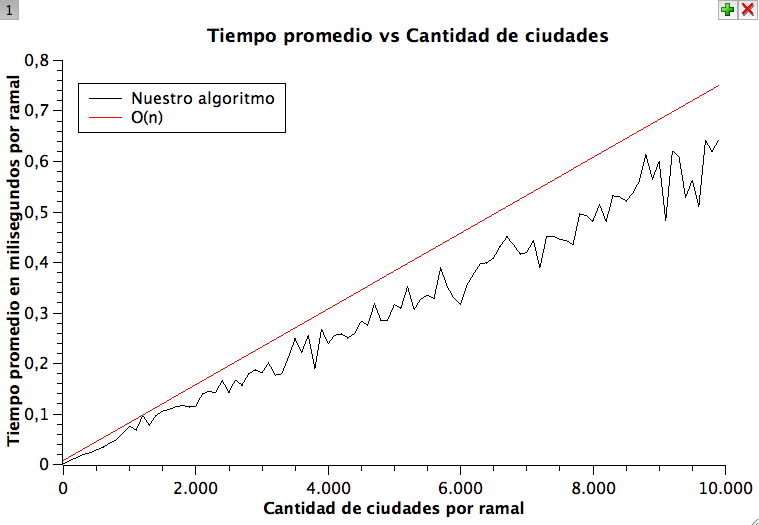
\includegraphics[width=\linewidth]{../graficos/ej1/TIempoPromedioVsCantidadCIudades.png}
  \caption{{\small Comparación con O(n). Dado un archivo de entrada con longitud de cable y kilometrajes de estaciones random.}} \label{ej1-tiempo-vs-cant-ciudades-random}
\endminipage

\end{center}
\end{figure}


\subsubsection{Peor caso}

El próximo test generado consiste en tener una ciudad al final muy lejos, lo que produciria que ``actual" $ $ llegue hasta el anteultimo, luego start lo alcance y esto produzca que se pase por todas las ciudades dos veces. Esto lo consideramos un Peor caso ya que el resto de los casos no haces falta pasar dos veces por todas las ciudades.  Para probar esto, escribimos un script que nos asegure que la ultima ciudad este muy alejada. En cuanto a las estaciones del ramal, configuramos números random y el ultimo muy grande. Estos archivos se encuentran en la carpeta ``Ejercicio 1" $ $ con prefijo ``2doEjemplo", y``generadorArchivosInRandom.py" $ $es el script con los distintos tests, comentados. Veamos un ejemplo:\\

\begin{itemize}
\item La longitud del cable no alcanza para conectar ninguna ciudad:\\
\textbf{in:}\\
1\\
3 6 8 12 15 20 24 49 58 70 90 123 \\
\textbf{out:}\\
0\\

En este caso la longitud del cable es 1, y todas las distancias son mayores que 1, por lo tanto está bien que nuestro algoritmo devuelva que conectó 0 ciudades.\\
\end{itemize}

\begin{figure}[H]
\begin{center}

\minipage{0.8\textwidth}
  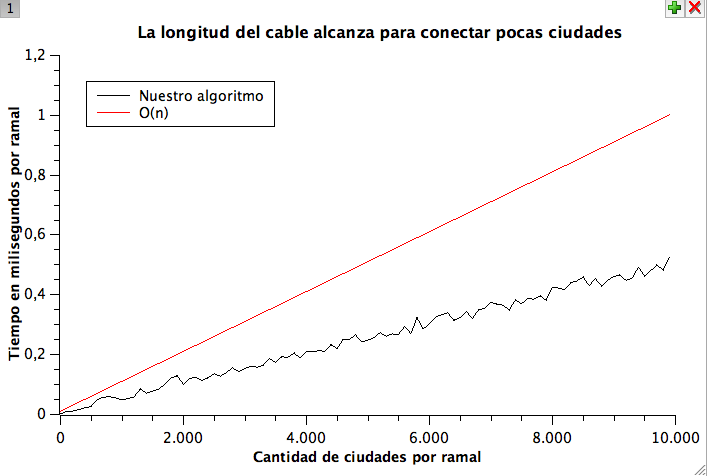
\includegraphics[width=\linewidth]{../graficos/ej1/CableCorto.png}
  \caption{{\small Comparación con O(n). Dado un archivo de entrada con un cable corto y kilometrajes de estaciones random.}} \label{ej1-tiempo-vs-cant-ciudades-random-long-cable-1}
\endminipage

\end{center}
\end{figure}

En la figura \ref{ej1-tiempo-vs-cant-ciudades-random-long-cable-1} vemos como nuestro algoritmo sigue respentando el límite de complejidad propuesto por la cátedra, a pesar de que éste sea un caso ``border". \\

\subsubsection{Mejor caso}

Otro test que decidimos hacer fue el caso contrario a este, que sería tener un cable demasiado largo, que permita conectar todas las ciudades de los ramales. Esto lo consideramos como el mejor caso, ya que al tener un cable suficientemente largo como para conectar todas las ciudades, el primer puntero ($"$start$"$) no es necesario que se mueva, solo avanza el segundo. Para ver esto , escribimos un script de manera tal que la cantidad de kilómetros de cable siempre supere la distancia entre la primera ciudad y la ciudad del último kilómetro del ramal. Al medir los tiempos promedios vemos que nuestro algoritmo sigue tardando menos que O(n), y lo podemos observar en la figura que sigue, pero antes veamos un ejemplo. \\

\begin{itemize}
\item El cable alcanza para conectar todas las ciudades:\\
\textbf{in:}\\
10000\\
1 4 67 78 90 95 120 150 270 380 456 900 1300 1809 5546 8403\\
\textbf{out:}\\
17\\
\end{itemize}
En este caso al tener un cable de longitud = 10000km y todas las estaciones estar a distancia menor que 10000km, el algoritmo devuelve 17 que son la cantidad de estaciones del ramal + la ciudad de kilómetro 0, pues la distancia entre ésta ciudad y la primera es de 1km. Veamos el grafico \ref{ej1-tiempo-vs-cant-ciudades-random-long-cable-largo}. \\

\begin{figure}[H]
\begin{center}

\minipage{0.8\textwidth}
  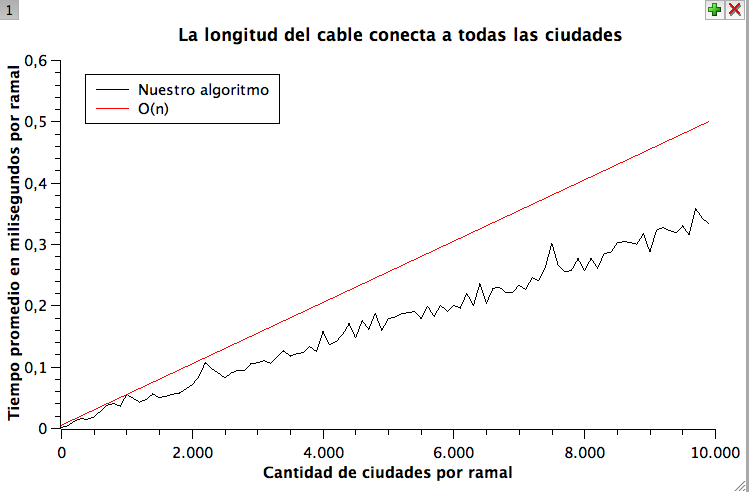
\includegraphics[width=\linewidth]{../graficos/ej1/CableLargo.png}
  \caption{{\small Comparación con O(n). Dado un archivo de entrada con un cable muy largo y kilometrajes de estaciones random.}} \label{ej1-tiempo-vs-cant-ciudades-random-long-cable-largo}
\endminipage

\end{center}
\end{figure}

\subsubsection{Peor caso vs Mejor caso vs O(n)}

A continuación ilustramos un gráfico en donde comparamos el tiempo que tarda el algoritmo en el mejor caso, con el tiempo del peor caso y con O(n). Para realizar el gráfico definimos la línea O(n) como n $*$ 0,01.

\begin{figure}[H]
\begin{center}

\minipage{0.8\textwidth}
  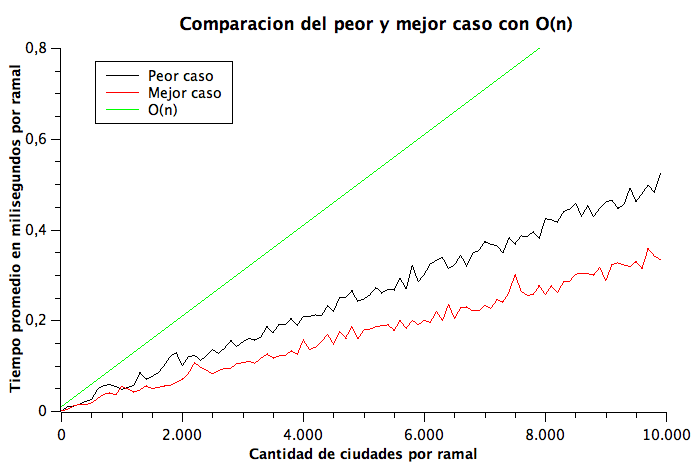
\includegraphics[width=\linewidth]{../graficos/ej1/PeorYMejorCasoVsOn.png}
  \caption{{\small Comparación con O(n) del mejor y peor caso anteriormente explicados. }} \label{ej1-tiempo-vs-cant-ciudadades-mejor-peor-caso}
\endminipage

\end{center}
\end{figure}


\subsubsection{Otros casos interesantes:}
\begin{itemize}
\item Cuando el cable alcanza para conectar solo las primeras ciudades:\\
\textbf{in:}\\
9\\
1 2 3 4 5 40 55 68 79 99 130 139 200 259 2889\\
\textbf{out:}\\
6\\

\end{itemize}

Al tener un cable de longitud 9km, las primeras 5 estaciones estar a 1 kilómetro de distancia entre ellas, y las siguientes distancias superar los 9km, si contamos estas 5, y a la ciudad del kilómetro 0, no devuelve las 6 ciudades que conecta.\\

\begin{figure}[H]
\begin{center}

\minipage{0.8\textwidth}
  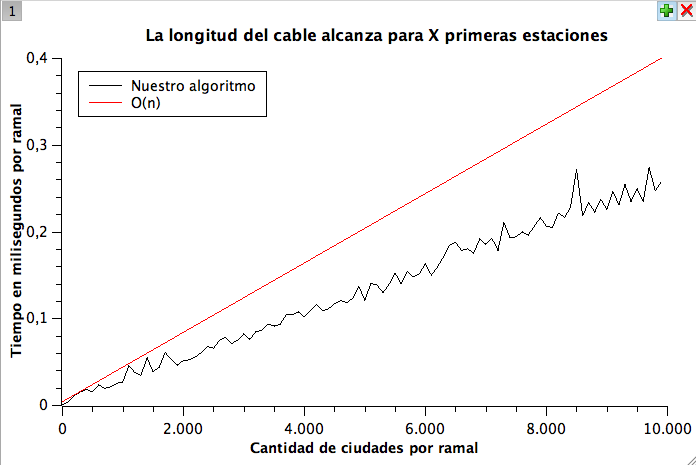
\includegraphics[width=\linewidth]{../graficos/ej1/PrimerasCiudades.png}
  \caption{{\small Comparación con O(n). Dado un archivo de entrada donde entre las primeras ciudades hay una distancia corta.}} \label{ej1-tiempo-vs-cant-ciudadades-primeras-ciudades}
\endminipage

\end{center}
\end{figure}
\begin{itemize}
\item Cuando el cable alcanza para conectar sólo las últimas ciudades:\\
\textbf{in:}\\
8\\
10 20 35 47 82 99 120 143 155 200 267 298 299 300 301\\
\textbf{out:}\\
4\\
\end{itemize}

Al ser un cable de longitud 8km, y las primeras 12 estaciones estar a distancia mayor que 8km, no conecta ninguna de ellas, pero si lo hace con las últimas 4 ya que la distancia de las mismas es menor que 8km. \\

\begin{itemize}
\item Cuando por 1 kilómetro, el cable no alcanza y no se conectan ciudades:\\
\textbf{in:}\\ 
3\\
4 8 12 16 20 24 28 32 \\
\textbf{out:}\\
0\\

La distancia entre todas las estaciones es de 4km, y el cable tiene un largo de 3km, por lo tanto, al faltarle siempre 1km para poder conectar al menos dos ciudades, devuelve 0. Esto es correcto ya que no alcanza el cable y no ``conecta" ciudades. \\

A continuación mostramos el gráfico que resulta de medir el tiempo que tarda el algoritmo al correr un archivo de entrada que generamos con ciudades que están a una distancia: longitud del cable + 1 y compararlo con O(n), en particular para este ejemplo, lo comparamos con 0,006 $*$ O(n). Los archivos que usamos son: ``generadorArchivosInRandom.py" (ejemplo 6), ``6toEjemploTiempoEnMilisegundos.txt", \\ ``6toEjemploPor1KmNoAlcanza.in", ``6toEjemploPor1KmNoAlcanza.out" y , ``ejemploTamCiudades.txt"\\

\end{itemize}

\begin{figure}[H]
\begin{center}

\minipage{0.8\textwidth}
  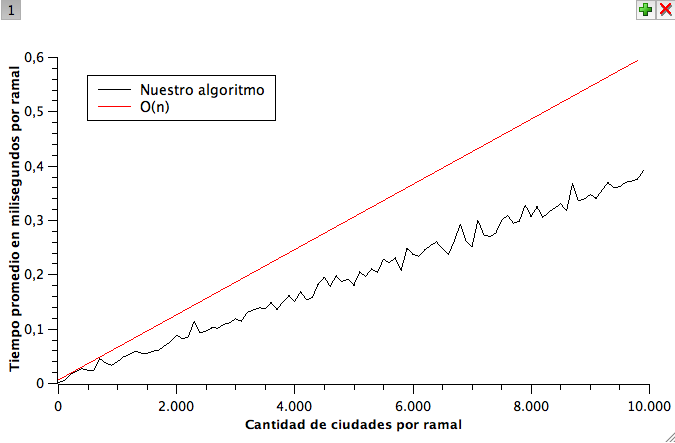
\includegraphics[width=\linewidth]{../graficos/ej1/falta1KmSiempre.png}
  \caption{{\small Comparación con O(n). Dado un archivo de entrada donde siempre falta 1 km para conectar las ciudades.}} \label{ej1-tiempo-vs-falta-1-km-siempre}
\endminipage

\end{center}
\end{figure}

